\section*{Качество классификации: Precision, Recall}

В задаче классификации \textbf{precision} (точность) и \textbf{recall} (полнота) являются ключевыми метриками для оценки качества предсказания, особенно в задачах с несбалансированными классами.

\subsection*{Определения}

Рассмотрим бинарную классификацию, то есть объект может быть либо положительным (positive), либо отрицательным (negative), и определим:

\begin{itemize}
    \item $TP$ (\textit{True Positives}) — количество объектов, правильно классифицированных как положительные.
    \item $FP$ (\textit{False Positives}) — количество объектов, ошибочно классифицированных как положительные.
    \item $FN$ (\textit{False Negatives}) — количество объектов, ошибочно классифицированных как отрицательные.
    \item $TN$ (\textit{True Negatives}) — количество объектов, правильно классифицированных как отрицательные.
\end{itemize}

На основе этих величин вычисляются:

\begin{enumerate}
    \item \textbf{Precision:}
    \[
    \text{Precision} = \frac{TP}{TP + FP}.
    \]
    Precision показывает долю истинно положительных объектов среди всех объектов, классифицированных как положительные.

    \item \textbf{Recall:}
    \[
    \text{Recall} = \frac{TP}{TP + FN}.
    \]
    Recall показывает долю истинно положительных объектов среди всех реально положительных объектов.
\end{enumerate}

\begin{figure}[ht!]
	\centering
	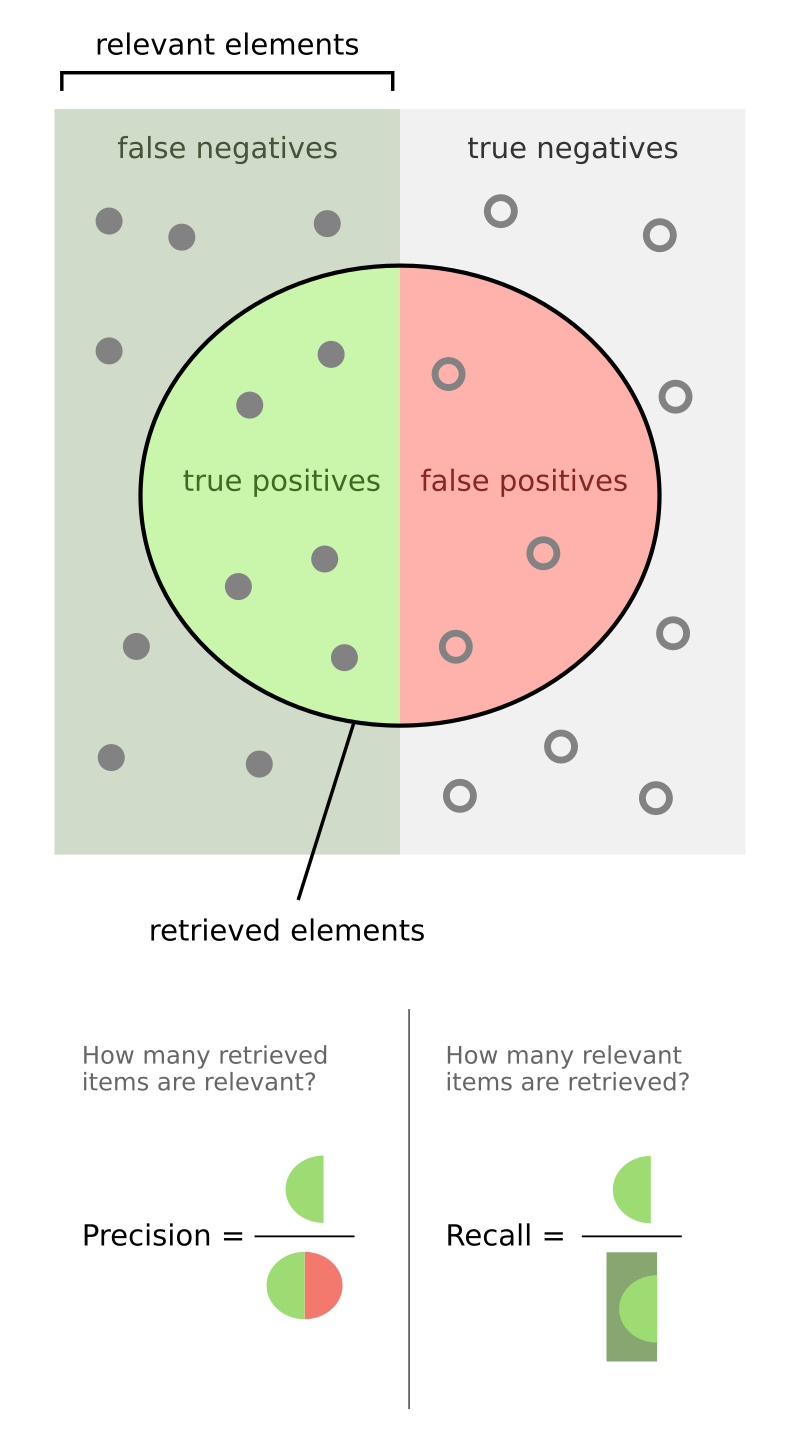
\includegraphics[width=0.65\linewidth]{chapters/model_selection/images/Precisionrecall.png}
\end{figure}

\subsection*{Интуитивное объяснение}

\begin{itemize}
    \item \textbf{Precision}: Насколько «точен» алгоритм, когда он говорит, что объект положительный? Если precision высокое, значит, ложные срабатывания ($FP$) минимальны.
    \item \textbf{Recall}: Насколько хорошо алгоритм находит все положительные объекты? Если recall высокое, значит, пропущенные положительные объекты ($FN$) минимальны.
\end{itemize}

\subsection*{Пример}

Классический пример использования метрик precision и recall - задача поиска спама на почте. В этом случае спам - положительная категория. Пусть у нас есть 100 писем, из которых 40 писем — спам, 60 писем — не спам.

Алгоритм классифицировал 50 писем как спам, из которых 30 писем действительно оказались спамом, а остальные 20 писем были ошибочно классифицированы как спам. Вычислим в этом случае precision и recall:

\begin{itemize}
    \item \textbf{Precision:}
    \[
    \text{Precision} = \frac{TP}{TP + FP} = \frac{30}{30 + 20} = 0.6.
    \]

    \item \textbf{Recall:}
    \[
    \text{Recall} = \frac{TP}{TP + FN} = \frac{30}{30 + 10} = 0.75.
    \]
\end{itemize}

\subsection*{Баланс между precision и recall}

Модель для каждого объекта на входе генерирует какое-то число на выходе. В простейшем варианте объект классифицируется как положительный, если это число больше некого выставленного порога, и как отрицательный в обратном случае. Увеличивая порог классификации, мы снижает количество False Positive объектов, потому precision увеличивается. При этом количество "незамеченных" моделью положительных объектов тоже вырастет, поэтому recall снизится. При уменьшении порога будет наблюдаться обратный эффект. Обычно стараются добиться компромиссного значения, при котором precision и recall оба принимают удовлетворительные значения. В некоторых случаях одна из метрик важнее другой:

\begin{itemize}
    \item Детекция спам-рассылок. В этом случае мы чаще всего не хотим пометить важные письма, как спам. Поэтому нужно снизить False Positive - важнее precision.
    \item Первичного выявление заболевания. Мы не хотим пропустить пациентов, которые на самом деле больны, только потому что модель сказала обратное. Поэтому важно снизить False Negative - в этом случае важнее recall. 
\end{itemize}

\subsection*{Интуитивное объяснение}

Если при получении положительного ответа от модели мы предпринимаем какое-либо действие, то precision важнее, когда действие обходится дорого, а recall важнее, когда бездействие обходится дорого. В примерах выше: помещение важного письма в папку "спам" (действие) может привести к финансовым потерям, а пропуск реального спама во "входящие" (бездействие) лишь заставит человека сделать это вручную. С другой стороны, при ложноположительном диагнозе человек пройдёт дополнительные анализы (действие), а ложноотрицательный может стоить ему жизни (бездействие).

\begin{figure}[ht!]
	\centering
	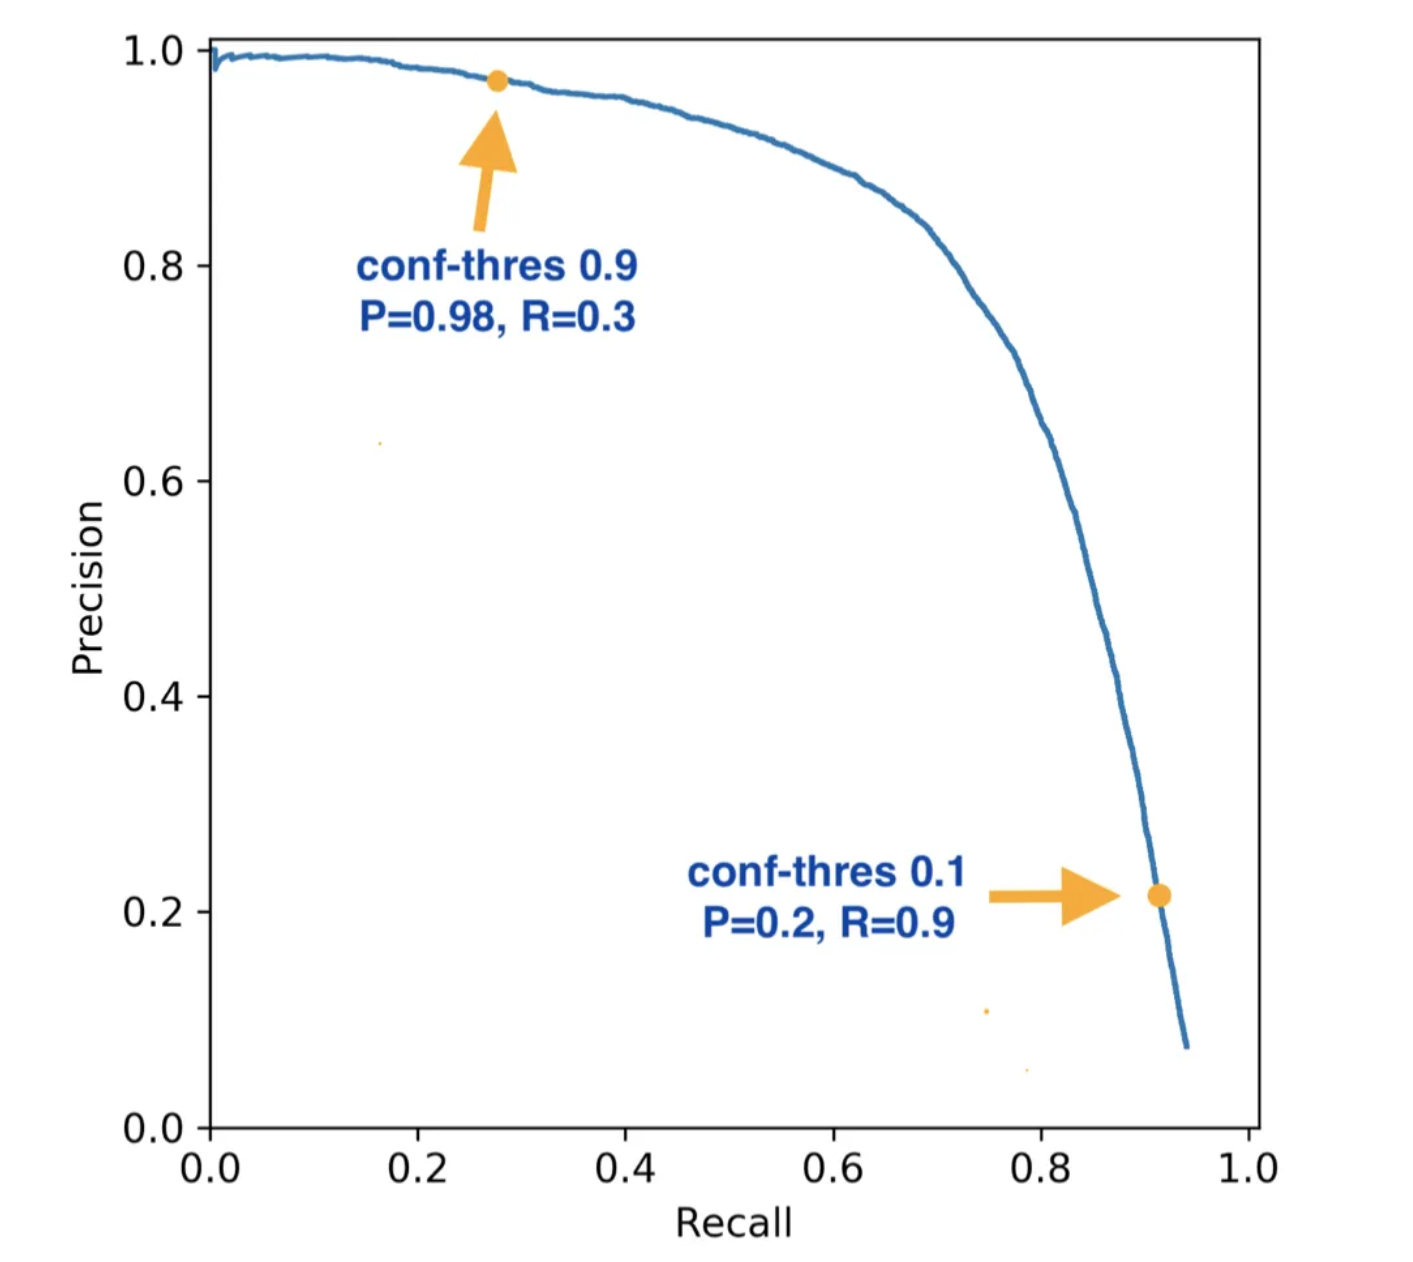
\includegraphics[width=0.65\linewidth]{chapters/model_selection/images/Precisionrecallcurve.png}
\end{figure}

\bigskip
\bigskip

Для того, чтобы изобразить баланс между двумя метриками, строят precision-recall кривую. Точки на ней соответствуют разным значениям порога.

\subsection*{F-метрика (дополнительно)}

Часто для оценки общего качества модели используется метрика $F$-мера, которая является гармоническим средним между precision и recall с параметром $\beta$:
\[
F_{\beta} = (1 + \beta^2) \cdot \frac{\text{Precision} \cdot \text{Recall}}{\beta^2 \cdot \text{Precision} + \text{Recall}}.
\]
Из формулы понятно, что $\beta$ определяет, насколько recall важнее по сравнению с precision. Наиболее часто используется $F_1$-мера:
\[
F_1 = 2 \cdot \frac{\text{Precision} \cdot \text{Recall}}{\text{Precision} + \text{Recall}}.
\]

\subsection*{Задачи}

\subsection*{Задача 1: Простейшая модель}

Как будет выглядеть precision-recall кривая у простейшей модели, которая для любого объекта делает positive предсказание с вероятностью $1-t$ (при $t = 1$ все предсказания отрицательные, при $t = 0.5$ - половина)? Как в этом случае и с использованием метрик precision и recall подбирать параметр $t$, чтобы добиться лучшей работы модели?

\textbf{Ответ:}

В координатах ($recall$, $precision$) - отрезок с концами в (0, $\alpha$) и (1, $\alpha$), где $\alpha$ - доля положительных объектов в выборке (горизонтальный отрезок). Объяснение состоит в том, что доля $TP$ равна $\alpha (1-t)$, доля $TP + FN$ равна $\alpha$, а доля $TP + FP$ равна $(1-t)$. Таким образом, значения precision и recall не зависят от параметра $t$, то есть его изменение не изменит качество модели в этих метриках.

\subsection*{Задача 2: Дисбаланс классов}

Какая из метрик -- precision или recall -- будет больше в случае сильного дисбаланса классов на тестовой выборке (рассмотреть оба случая), если известно, что модель обучалась на сбалансированном датасете?

\textbf{Ответ:}

Если положительных объектов значительно меньше, чем отрицательных, то recall будет больше. Это связано с тем, что сбалансированная модель в этом случае будет допускать много False Positive ошибок. При обратном дисбалансе precision будет больше из-за большого количества False Negative ошибок.

\subsection*{Задача 3: Мошеннические транзакции}

Финансовая компания использует алгоритм для выявления мошеннических транзакций. Из 10,000 проверенных транзакций 500 транзакций являются мошенническими, 9,500 транзакций являются легитимными.

Алгоритм определил 600 транзакций как мошеннические, из которых 400 действительно оказались мошенническими.

\begin{enumerate}
    \item Вычислите $F_1$-меру.
    \item Насколько может измениться $F_1$-мера, если алгоритм пометит ещё 50 транзакций как мошеннические, в зависимости от того, являются они на самом деле мошенническими или нет?
\end{enumerate}

\textbf{Решение:}
Найдём precision и recall.
\begin{itemize}
    \item
    \[
    \text{$precision$} = \frac{400}{400 + 200} = \frac{400}{600} \approx 0.667.
    \]
    \item
    \[
    \text{$recall$} = \frac{400}{400 + 100} = \frac{400}{500} = 0.8.
    \]
    \item
    \[
    \text{$F_1$-score} = 2\frac{precision\cdot recall}{precision + recall} = 2\frac{0.667\cdot 0.8}{0.667 + 0.8} \approx 0.722
    \]

\end{itemize}

Обозначим за $\alpha$ долю тех новых помеченных транзакций, которые на самом деле являются мошенническими ($0 \le \alpha \le 1$). Понятно, что $TP$ увеличится на $50\alpha$, $FN$ уменьшится на $50\alpha$, а $TP + FP$ станет равным 650. Посчитаем precision, recall, изменение $F_1$-score в общем случае:

\begin{itemize}
    \item
    \[
    \text{$precision$} = \frac{400 + 50\alpha}{650}.
    \]
    \item
    \[
    \text{$recall$} = \frac{400 + 50\alpha}{500}.
    \]
    \item
    \[
    \text{$F_1$-score} = \frac{16 + 2\alpha}{23} \approx 0.696 + 0.087\alpha
    \]
    \item
    \[
    \text{$\Delta F_1$-score} \approx 0.696 + 0.087\alpha - 0.722 = -0.026 + 0.087\alpha
    \]
\end{itemize}

Таким образом, $F_1$-мера уменьшится на -0.026 если все новые помеченные транзакции на самом деле легитимные, увеличится на 0.061, если они все на самом деле мошеннические. Заметим, что $F_1$-мера останется неизменной, если $\alpha = \frac{1}{3}$, то есть изначальная доля ложноположительных среди всех помеченных.


